\documentclass[20 pts]{article}
%\usepackage{xeCJK}
\usepackage{amsfonts}
\usepackage{amssymb}
\usepackage{csvsimple}
\usepackage{caption}
\usepackage{longtable}
\usepackage{amsmath}
\usepackage{bm}
\usepackage{graphicx}
%\setCJKmainfont{SimSun}
\title{Deterministic Interleaver Design for Turbo Codes} 
\author{Kwame Ackah Bohulu, 1631133}
\date{22-06-2017}


\begin{document}
\maketitle
\newpage
\section{Abstract}
input weight 2m error events with the distance between the bit '1' seperated by a 
multiple of
the componet codes cycle length ($a-\tau$ seperated input weight 2m error events) 
tend to produce low-weight turbo codewords if present
in both component codes. In this research paper, we introduce a 
method for designing deterministic
interleavers for turbo codes in such a way that $a-\tau$ seperated input weight 2m error events in 
the first component encoder are not mapped unto the second component encoder. 
Using
this method, we find good interleavers for specified frame lengths and component 
codes. The performance of the designed interleavers is tested against the Quadratic 
Permutation Polynomial (QPP) Interleaver and is shown to be better especially for long
frame sizes.

\section{Introduction}
Turbo Codes are amongst the class of capacity approaching FEC codes that were 
discovered in 1993 by Claude Bearoux. They are constructed by the parallel 
concatenation of 2 Recursive Systematic Convolutional (RSC) Encoders via an interleavers. Diagram for 


Decoding of Turbo codes is done using the Turbo Decoder. It is made up 2 Soft Input Soft 
Output (SISO) Decoders.
The interleaver plays a very important role in Turbo codes as it reduces the number of
 low-weight codewords(multiplicity) of the Turbo code [4]. However, the existence of 
 the low-weight codewords causes the turbo codes to have a high error floor in the 
 high SNR region. A lot of research has been done concerning interleavers for 
 turbo codes and they are generally put into 2 groups, Random and 
 Deterministic interleavers.
\paragraph{}
Turbo codes implemented using Random interleavers have been shown to have good
 performance, especially for large frame sizes [3]. The disadvantage of using 
 Random interleavers stems from required use of interleaver tables in both the 
 encoder and decoder, which is undesirable in many applications. Deterministic interleaver
  on the other hand require no such interleaver tables and the logic behind interleaving
   and deinterleaving can be executed by means of algorithms. Due to this advantage, 
   a lot of Turbo codes employ Deterministic interleavers in their construction. Most 
   noticable amongst these is the Quadratic Permutation Polynomial (PP2) interleaver [3]
    which is used in LTE applications.
\paragraph{}
Despite this advantage, Deterministic interleavers that outperform Random interleavers,
 especially for large frame sizes have yet to be discovered. The aim of this research is
  to design an interleaver that has a performance that is at least as good as that of random 
  interleavers for large frame sizes. 

\subsection{Turbo Encoding and Decoding}
The Turbo encoder is shown in figure (\ref{TC}).

\begin{center}
\begin{figure}[h!]
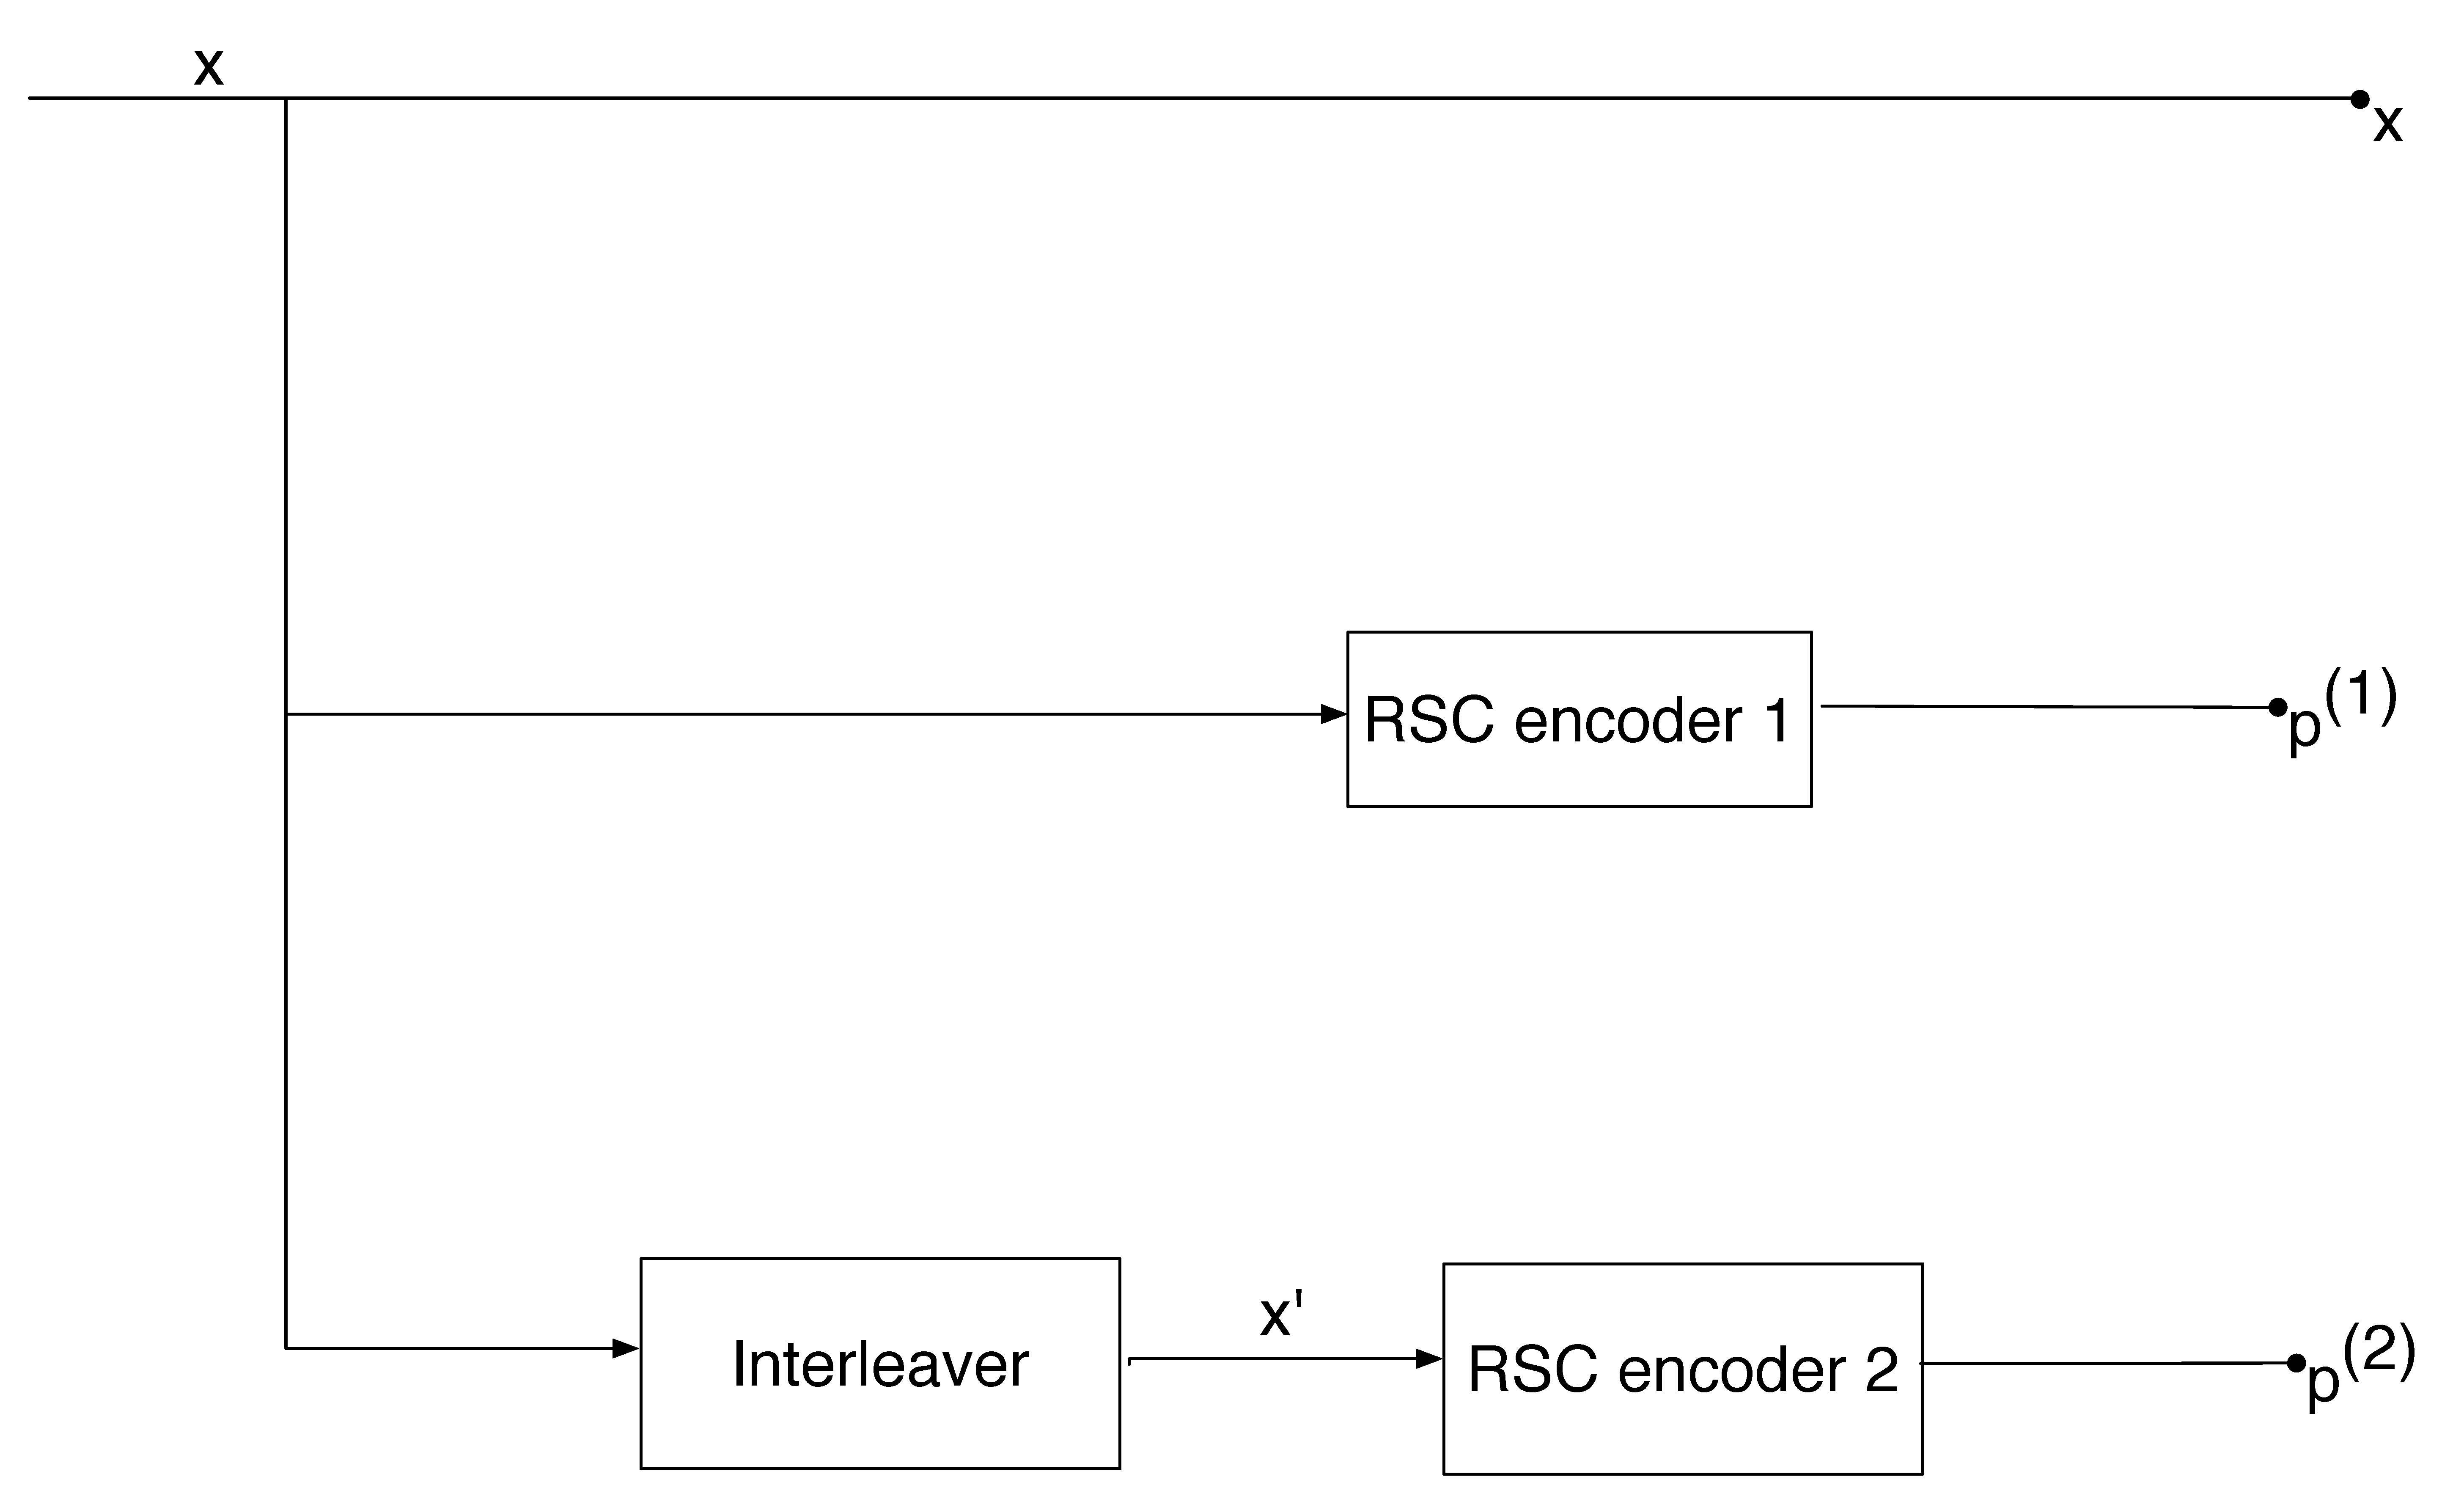
\includegraphics[width=8cm]{TurboEncoder.pdf}
\caption{Turbo Encoder}
\label{TC}
\end{figure}
\end{center}

The input information bits of length N is fed into the first RSC encoder which produces the
first parity check bits. The input to the second RSC encoder is an interleaved version 
input information bits and this is used to generate the second parity check bits. Both parity
check bits have length N which gives an output rate of 1/3.The RSC encoders used are known as component encoders. Usually identical component
encoders are used.
\paragraph{}
Decoding of Turbo Codes is done using the Turbo Decoder which is made up of 2 Soft Input
Soft Output (SISO) decoders. The Turbo decoder is shown in (\ref{TD}).
\begin{figure}[h!]
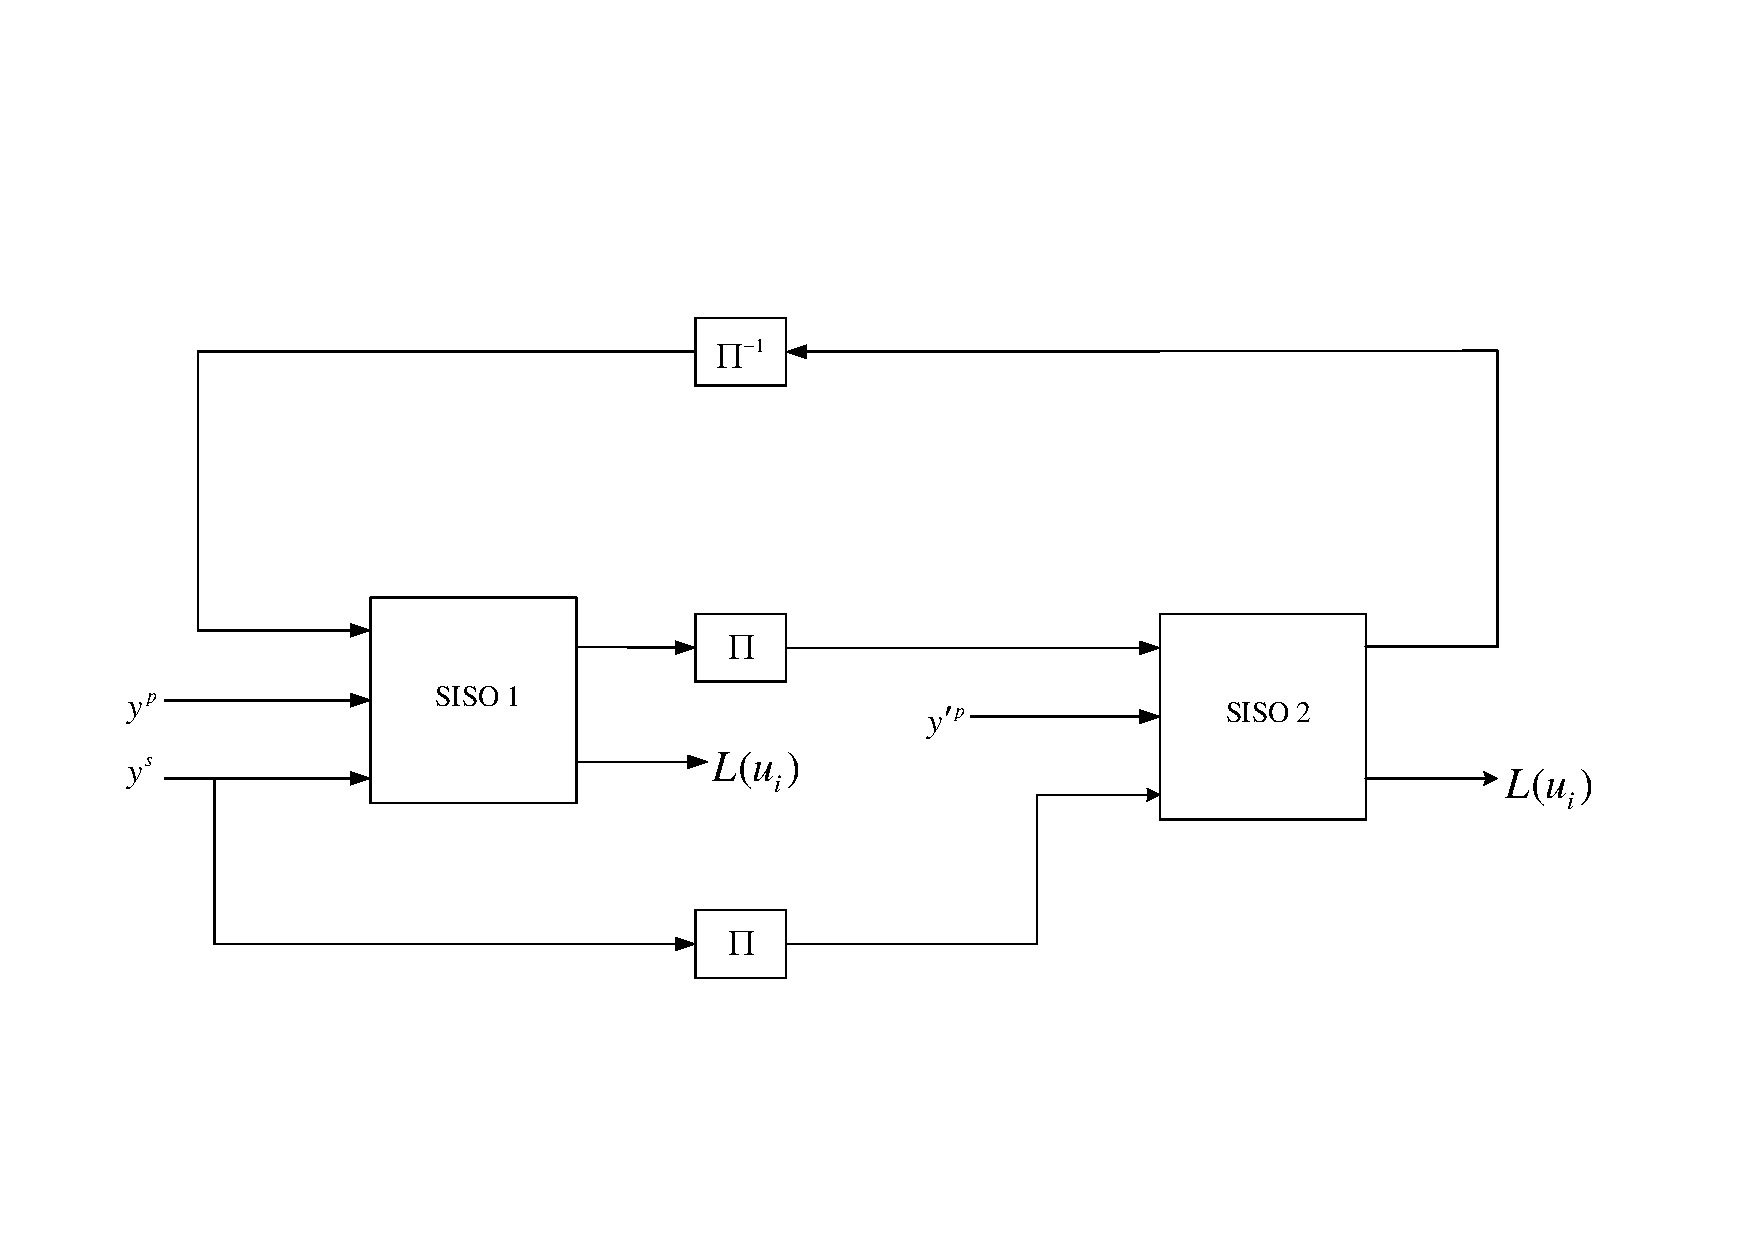
\includegraphics[width=10cm]{D1.pdf}
\caption{Turbo Decoder}
\label{TD}
\label{図2}
\end{figure}
An iterative decoding scheme based on the BCJR algorithm
is employed in the decoding of turbo codes.




The turbo decoding process is as follows
\paragraph{1}
The input to the first component decoder is $(\boldsymbol{y}^s,\boldsymbol{y}^p)$ and relates
 to the systematic bits and the parity bits of the first component encoder of the Turbo encoder.
\paragraph{2}
The Log-Likelihood Ratio (LLR),$L(u_i)$ is calculated. For the first iteration, it is assumed 
that the input information bits have equal probability and the a-priori LLR value 
$L^{(a)}(u_i)$ is set to 0。
\paragraph{3}
At the output of the first componet decoder, the channel LLR values, $L_cy_i^s$ is subtracted from $L(u_i)$ to yield the extrinsic LLR values 
of the first component decoder, $L_{12}^{(e)}(u_i)$. $L_{12}^{(e)}(u_i)$ is then interleaved and fed into the second component decoder as the value for $L^{(a)}(u_i)$.
\paragraph{4}
The other inputs to the second component decoder are $({\boldsymbol{y}'}^s,{\boldsymbol{y}'}^p)$ which
correspond to the interleaved systematic bits and the parity bits of the second component
encoder. These are used to calculate the extrinsic LLR values 
of the second component decoder,$L_{21}^{(e)}(u_i)$.
\paragraph{5}
$L_{21}^{(e)}(u_i)$ is deinterleaved、and fedback into the first component encoder as the new $L^{(a)}(u_i)$ value.
\paragraph{}
The iteration is either repeated for a predetermined number of times, or untill a certain condition is met. At the final iteration $L(u_i)$ (from the second component decoder)is deinterleaved and used to estimate the value of$u_i$.


\section{Methodology}
Turbo codes have error floor in the high SNR region. This has been attributed to the 
prescence of low-weight codewords. The error floor of the Turbo codes can be raised
 by increasing the interleaver size whiles maintaining the effective free distance. 
 Alternatively increasing the effective free distance of the Turbo while maintaining the 
 multiplicity serves a similar purpose [2]. The effective free distance of a code is the
  minimum distance associated with an input of weight 2. 
\paragraph{}
In RSC encoders, weight 2 inputs of the form $(1+D^{t\tau})(D^u) ,0\leq u\leq N-\tau, t=\{1,2,3,...\}$
 tend
 to produce low-weight codeword [1]. $\tau$ is the cycle length of the RSC encoder. 
 We shall call such low-weight producing weight 2 inputs $a-\tau$-seperated input 
 weight 2 errors. If the $a-\tau$-seperated input weight 2 errors are input into the 
 Turbo codes component encoders a low-weight codeword will be produced. 

To increase effective free distance of the turbo code, we design an interleaver in such 
a way that the input to the second is of the form 
\begin{equation}
(1+D^{c\tau})(D^u) ,0\leq u\leq N-\tau
\label{one}
\end{equation}
where $c$ is a large number.

\subsection{Linear interleaver design}
The mapping function for the linear interleaver is given by
\begin{equation}
\Pi_{\mathbf{L}_n}(i) \equiv bi  \mod N, \ 0 \leq i \leq N
\label{two}
\end{equation}
where $b$ is a positive integer that is co-prime to $N$. 
The simplest $a-\tau$-seperated input weight 2 error (t=1) is shown in the figure 
below.

\begin{center}
\begin{figure}[h!]
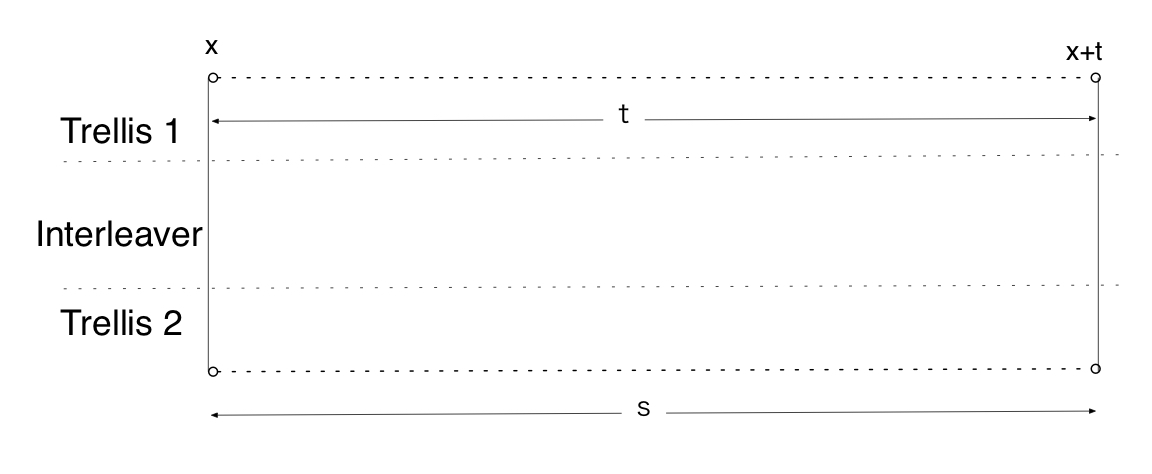
\includegraphics[width=8cm]{weight2.jpg}
\caption{$t=s=\tau$のエラーイベント}
\label{2_error}
\end{figure}
\end{center}

$s$ is calculated using the equation below.
\begin{equation}
\begin{split}
s&=\Pi_{\mathbf{L}_n}(x+t)-\Pi_{\mathbf{L}_n}(x)\\
&=b(x+t)-b(x) \mod N\\
&=bt \mod N
\label{three}
\end{split}
\end{equation}

The weight of the codeword can be calculated using the equation below.
\begin{equation}
d_{(t_i,s_j)}=w_o\Bigg( 3+\Bigg( \frac{ \left|t_i\right|}{\tau} + \frac{ \left|s_j\right|}{\tau} \Bigg)\Bigg)
\label{four}
\end{equation}

Substituting (\ref{three}) into (\ref{four}) and rewriting $t$ as $\tau$ gives
\begin{equation}
d_{(t_i,s_j)}=w_o\Bigg( 3+\Bigg( 1+ \frac{ b\tau \mod N}{\tau} \Bigg)\Bigg)
\label{five}
\end{equation}

It should be noted that values of b that are considered should satisfy the condition
\begin{equation}
( (b\tau \mod N )\mod \tau ) \neq 0
\label{six}
\end{equation}

The process for choosing the value of b that changes the input to the second 
component encoder into the form in (\ref{one}) is outlined below.

\paragraph{1.} For a given value of $b$ , $\ 1 \leq b \leq N/2$ which 
satisfies (\ref{six}) and all possible inputs of the form $(1+D^{t\tau})(D^u) ,0\leq u\leq N-\tau, t=1$, 
calculate corresponding s using (\ref{three})
\paragraph{2.} Calculate the Hamming distance for the codeword using
 equation (\ref{four}) and select min $d_{(t_i,s_j)}$
\paragraph{3.}After min $d_{(t_i,s_j)}$ is selected for all possible values of b,
 the value of b which corresponds to max(min $d_{(t_i,s_j)_v}$)

\paragraph{}
The tables below show the values for b selected for $t=\tau$ and $t=2\tau$ for 
various frame sizes.
\csvautolongtable[
      table head=\caption{$N=2^{m}$, $m = \{10, 11, 12, 13, 14\} $, $t=\tau$}\label{tab:t1}\\\hline
               \csvlinetotablerow\\\hline
               \endfirsthead\hline
               \csvlinetotablerow\\\hline
               \endhead\hline
               \endfoot,
               respect all
               ]{t_tau_1.csv}
               
               \csvautolongtable[
      table head=\caption{$N=2^{m}$, $m = \{10, 11, 12, 13, 14\} $, $t=2\tau$}\label{tab:t2}\\\hline
               \csvlinetotablerow\\\hline
               \endfirsthead\hline
               \csvlinetotablerow\\\hline
               \endhead\hline
               \endfoot,
               respect all
               ]{t_tau_2.csv}


    
\section{References}
\paragraph{1}  Oscar Y. Takeshita, Member, IEEE, and Daniel J. Costello ,
''New Deterministic Interleaver Designs for Turbo Codes'',IEEE Trans. Inform. Theory,
 vol. 46,pp. 1988-2006,Nov. 2000\\
  \paragraph{2} L. C. Perez, J. Seghers, D. J. Costello, Jr., 
  ''A distance spectrum interpretation of turbo codes'', IEEE Trans. Inform. Theory,
   vol. 42, pp. 1698-1709, Nov. 1996.\\
\paragraph{3} Jing Sun, Oscar Y. Takeshita ”Interleavers for Turbo Codes Using 
Permutation Polynomials over Integer Rings”, IEEE Trans. Inform. Theory, vol. 51,
pp. 101 - 119 Jan. 2005\\
\paragraph{4} John G. Proakis, Masoud Salehi. ''Digital Communications'', 
Fifth Edition,Chapter 8, McGraw-Hill\\.

\end{document}